
\cleardoublepage
\chapter*{Introduction}
\markboth{that separateon}{Introduction}
\addcontentsline{toc}{chapter}{Introduction}

Although the Earth receives an average of about 300 kW/m2 from the Sun, it would be uninhabitable without the magnetosphere to protect it from the plasma solar flares that would strip away its atmosphere. 

The magnetosphere generated by inner layer rotatoin of of the earth, is a shield. The geomagnetic storm. Substorm are disturbances that can make its tail change. The reconnection is the underlying process that make the magnetic energy 

On Earth the objective of achieving fusion generated electricity by means of magnetically confined plasma devices 

The need of a twisted magnetic field lines for confinement. The two type of devices : tokamak and stellarator concepts to create those.

a paragraph on the triple product and beta parameter as well as the money.

The islands lower the but can also be usefull for divertor concept.

As \cite{imbert-gerard_introduction_2020} nicely points out, the complexity of the description of processes in a plasma may be tackled by considering different models that depend on the length and time scale. The single particle approach in a magnetic field, here introduce quickly.

diverted plasmas.

MAP: "With the aid of modern dynamical system theory, the structure of a 3D vector field can be comprehended and analyzed in terms of invariant manifolds [9, 10]."

"It is important to note that one of the fundamental measures of chaos, the Lyapunov exponent is not usually a good measure for transport. In Ref. 86, we said: The Lyapunov exponents give the rate at which a nice cat in a region of phase space turns into a mixed-up cat. The turnstile rate constants give the mean rate at which bits of the cat are transported to regions of the phase space"

many maps, strange attractors, standard map

\begin{figure}[h!]
    \centering
    \begin{subfigure}[t]{0.49\textwidth}
        \centering
        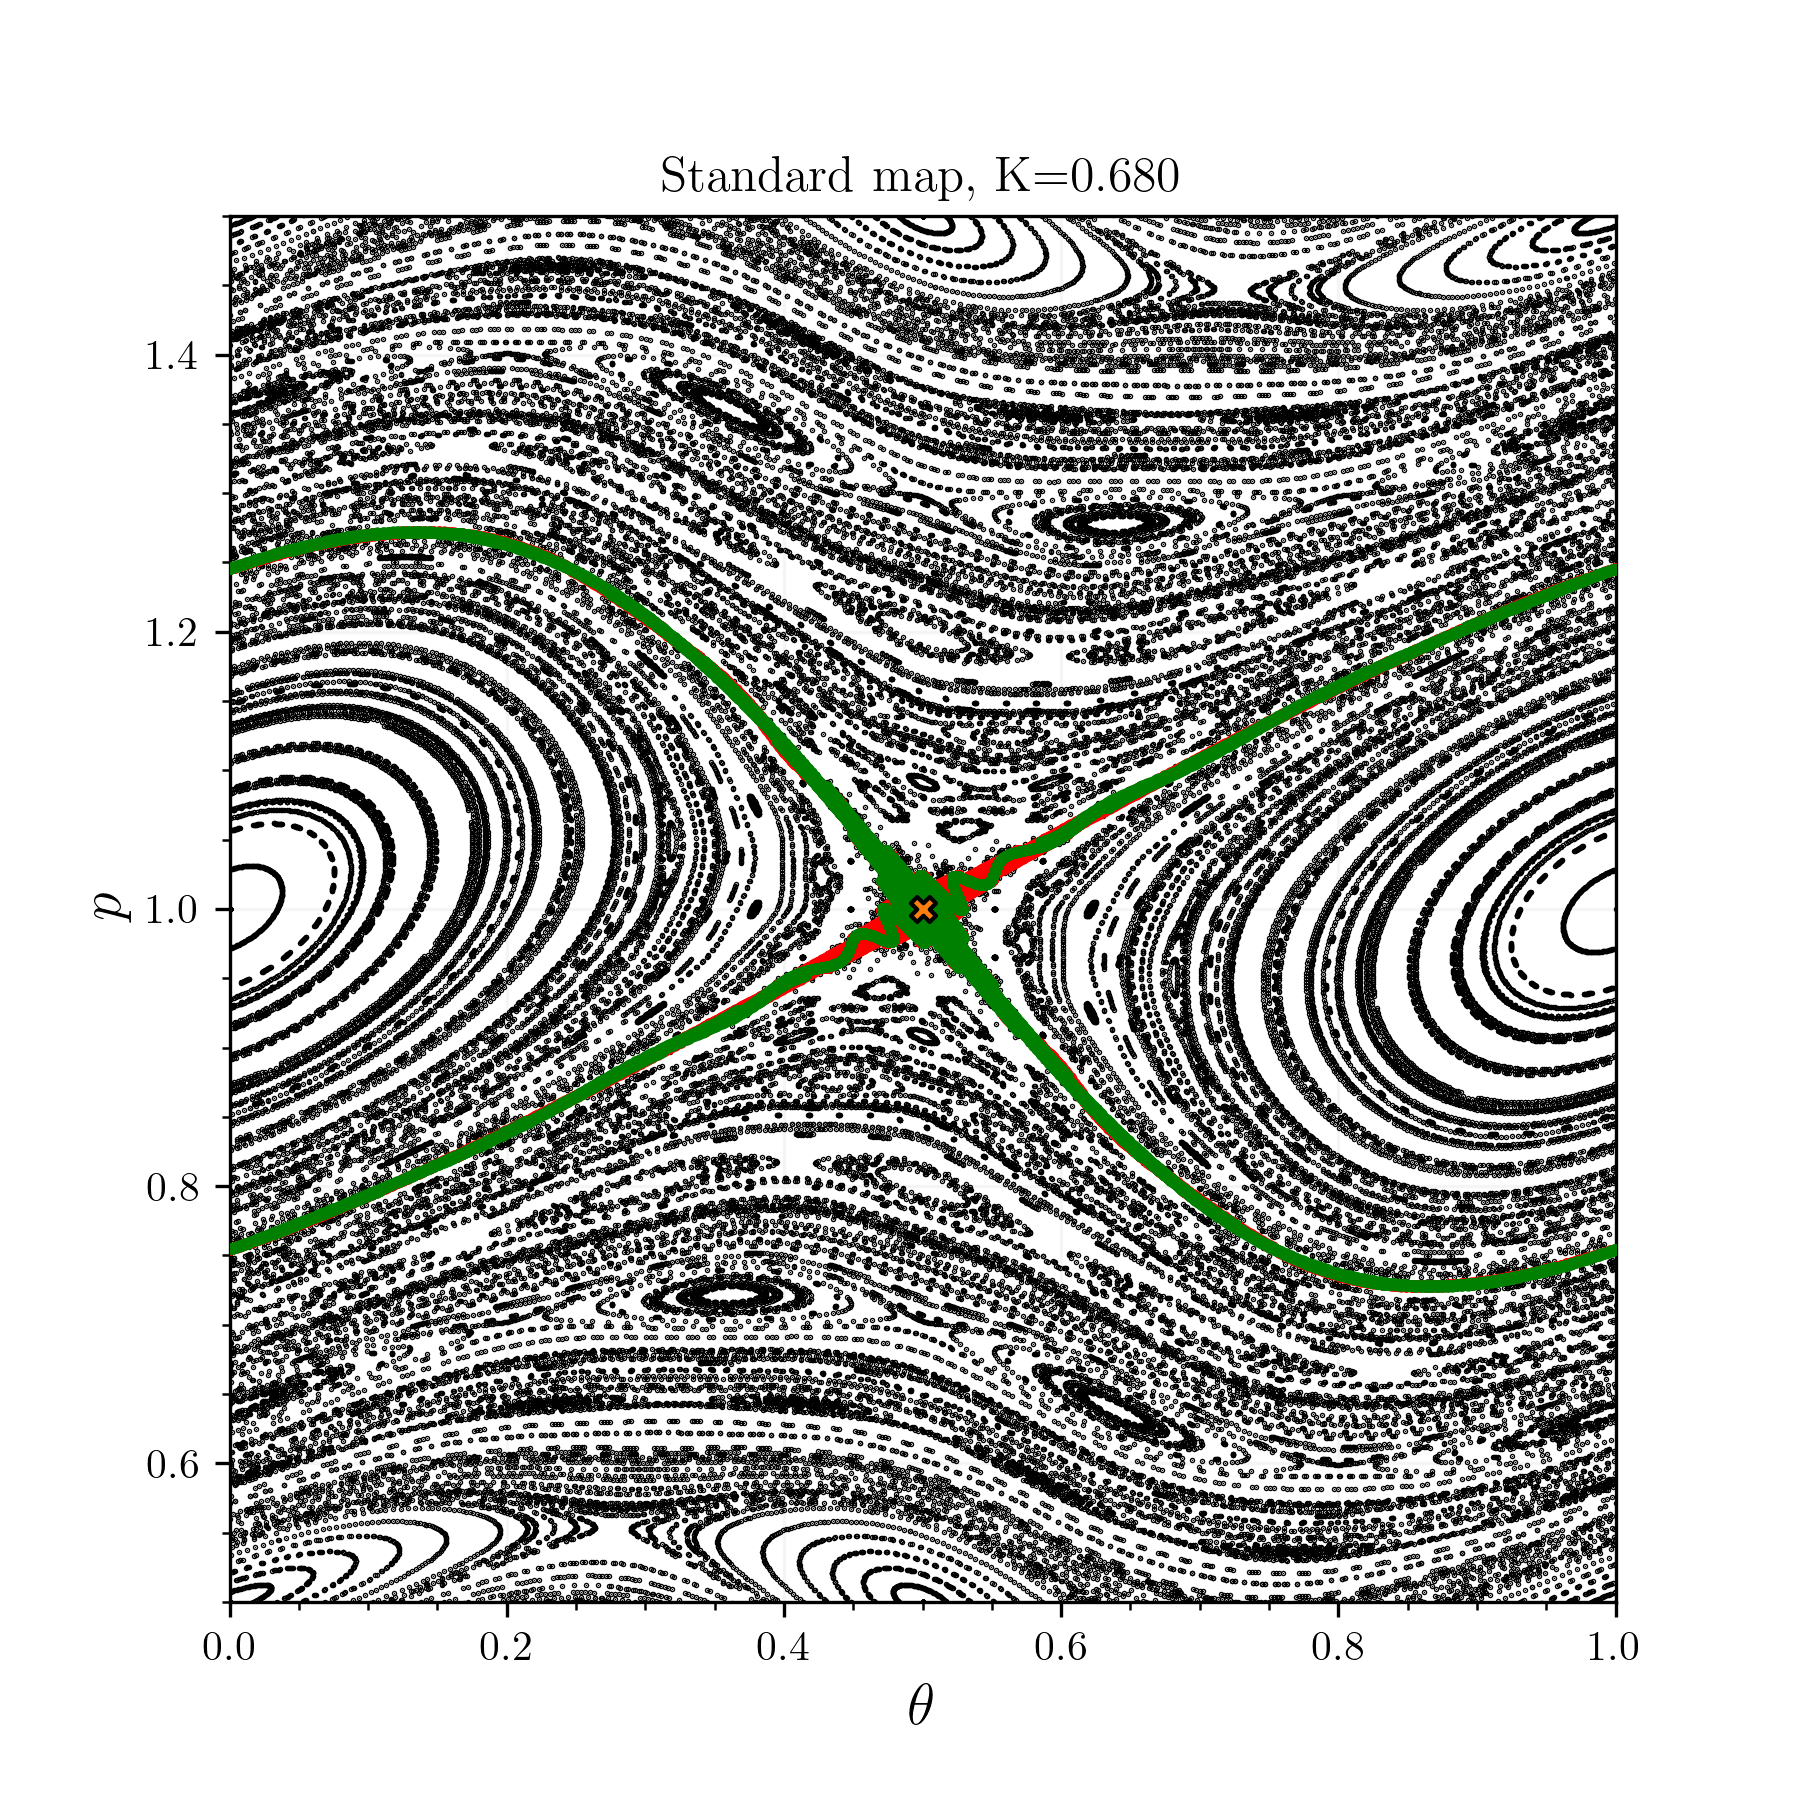
\includegraphics[width=\textwidth]{images/intro/manifold_0.680_28.png}
        \caption{}
        \label{fig:standard-map}
    \end{subfigure}
    \hfill
    \begin{subfigure}[t]{0.49\textwidth}
        \centering
        \includegraphics[width=\textwidth]{tok}
        \caption{}
        \label{fig:tokamap}
    \end{subfigure}
    \caption{Map for which the chaos is more easily studied and with similar behaviour with the field line chaos in the edge~: (a) standard map on the cylinder for the parameter $K=0.68$. (b) symmetric tokamap taken from \cite{wingen_stochastic_2005}.}
    \label{fig:mapping-the-chaos}
\end{figure}

\textbf{papers}:

\cite{meiss_thirty_2015} enlightens the progress that has been made in the characterization of transport for a deterministic dynamical system. Theoretical foundations in the context of volume-preserving maps (and therefore sympletic maps) are laid out ; the stable and unstable manifold of hyperbolic points bound resonance regions and their primary intersections, hetero/homo-clinic points, play an important role in determining the exiting/incoming fluxes. Inside chaotic layers, cantori are partial barriers separating orbits of the chaotic sea. Transition times are discussed and the fat fractal mixing of the islands for the Henon map is tackled down by considering a Markov chain decomposition.
\\[10pt]
In cylindrical geometry \cite{wei_invariant_2023} expose the link between field line tracing and the intersection with constant $\phi$ plane, Poincare section. The determinant of the Poincare map is related to the divergence of the vector field followed by the FLT. Two evolution to compute the manifold of hyperbolic fixed points, orbit of the Poincare map, are presented and an EAST shot combined with a RMP induced field shows the structure of the broken separatrix.

The continuous behaviour of the FLT needs to a discrete map is a non trivial problem.
However, the lack of an analytical formula for such a map, and hence the need to follow the field with the aid of an integrator, makes it difficult to look at the fine structure.
\\[10pt]
The Chirikov Standard map  
\\[10pt]
Restricting ourselves to the tokamak magnetic field, the tokamap has been introduced as a way of describing the FLT [ref]. Then [8] proposed a symmetric version of the map "based on a continuous Hamiltonian system consisting of an integrable part, specified by the safety factor, and a non-integrable perturbation". For monotinicaly increasing q-profile, \cite{wingen_stochastic_2005} analyses the escape rates due to the breaking of KAM surfaces and shows the presence of tangles. 
\\[10pt]
transoprt through chaos \cite{easton_transport_1991}
\\[10pt]
supressing stochasticity in stellarator \cite{hanson_elimination_1984}
\\[10pt]

\\[10pt]
Magnetic turnstiles in nonresonant stellarator divertor
\\[10pt]

experimental signatures of homoclinic tangles \cite{evans_experimental_2005}
\\[10pt]
For stellarators, the resonant divertor concept is based on the creation of islands at a specific $\Bar{\iota} = q^{-1}$ value to channel the flux at specific locations of the plasma-facing components. A non-resonant divertor, on the other hand, would not rely on this specific $q$ value, which can be difficult to achieve at the right location when bootstrap currents are present. \cite{garcia_exploration_2023} study the edge structure in the Compact Toroidal Hybrid device by analysing the connection length, and describe the effect of the chaotic behaviour on the trace left on a hypothetical divertor for varying current configurations and at different divertor positions using the EMC3-EIRENE 3D code. They calculate the heat flux and Mach number and make a parallel with the tangle structure that are present in ergodic divertors.
\\[10pt]
\cite{abdullaev_magnetic_2014} presents in more detail the magnetic stochasticity in magnetically confined plasmas and in particular the concept of the ergodic divertor. Initially used to correct inaccuracies of toroidal coils causing non-axisymmetric field in tokamaks, the resonant magnetic perturbation coils were also found usefull to mitagate ELM instabilities inherent of the H-mode, high confinment regime. The RMP coils are here discussed as a way to generate a stochastic (ergodic) region in the edge, controling the heat and particle fluxes and guiding particle towards the divertor plates. Ergodic divertors have been used in the WEST (formerly Tore Supra) and TEXTOR tokamaks.
\\[10pt]
mapping of stochastic field lines in poloidal divertor tokamaks \cite{abdullaev_mappings_2006}
\\[10pt]
poincare \cite{poincare_methodes_1892}
\\[10pt]
floer homology \cite{hohloch_homoclinic_2017}\cite{hohloch_transport_2012}

